


\tikzset{every picture/.style={line width=0.75pt}} %set default line width to 0.75pt        

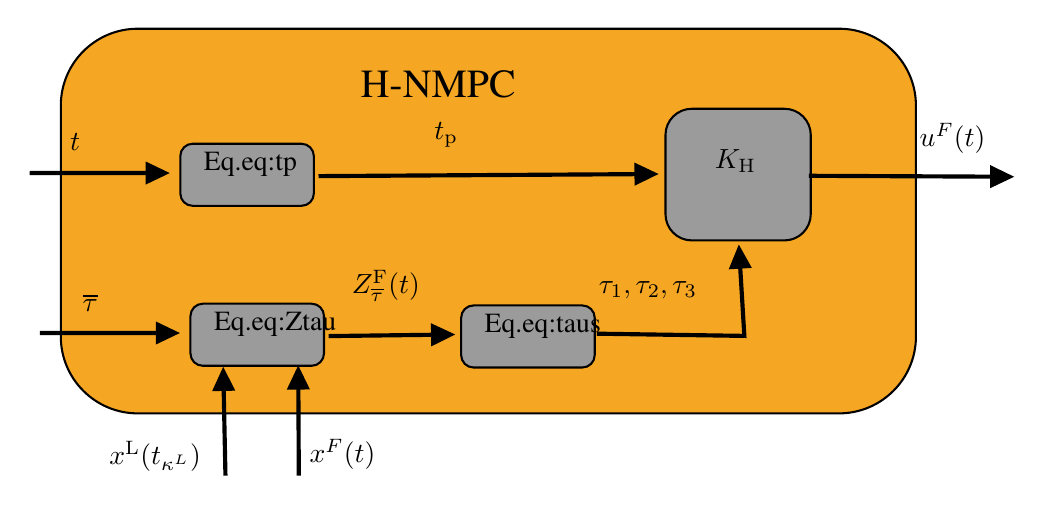
\begin{tikzpicture}[x=0.75pt,y=0.75pt,yscale=-1,xscale=1]
	%uncomment if require: \path (0,300); %set diagram left start at 0, and has height of 300
	
	%Rounded Rect [id:dp5342092506317702] 
	\draw  [fill={rgb, 255:red, 245; green, 166; blue, 35 }  ,fill opacity=1 ] (49,74.07) .. controls (49,53.6) and (65.6,37) .. (86.07,37) -- (423.93,37) .. controls (444.4,37) and (461,53.6) .. (461,74.07) -- (461,185.27) .. controls (461,205.74) and (444.4,222.33) .. (423.93,222.33) -- (86.07,222.33) .. controls (65.6,222.33) and (49,205.74) .. (49,185.27) -- cycle ;
	%Straight Lines [id:da7712511750690696] 
	\draw [line width=1.5]    (34.04,106.53) -- (97.47,106.54) ;
	\draw [shift={(101.47,106.54)}, rotate = 180.01] [fill={rgb, 255:red, 0; green, 0; blue, 0 }  ][line width=0.08]  [draw opacity=0] (11.61,-5.58) -- (0,0) -- (11.61,5.58) -- cycle    ;
	%Rounded Rect [id:dp43124631139892844] 
	\draw  [fill={rgb, 255:red, 155; green, 155; blue, 155 }  ,fill opacity=1 ] (340.33,88.25) .. controls (340.33,81.25) and (346.01,75.57) .. (353.02,75.57) -- (397.65,75.57) .. controls (404.65,75.57) and (410.33,81.25) .. (410.33,88.25) -- (410.33,126.31) .. controls (410.33,133.32) and (404.65,139) .. (397.65,139) -- (353.02,139) .. controls (346.01,139) and (340.33,133.32) .. (340.33,126.31) -- cycle ;
	
	%Rounded Rect [id:dp5272606094836356] 
	\draw  [fill={rgb, 255:red, 155; green, 155; blue, 155 }  ,fill opacity=1 ] (106.57,98.4) .. controls (106.57,95.1) and (109.25,92.42) .. (112.55,92.42) -- (164.94,92.42) .. controls (168.24,92.42) and (170.92,95.1) .. (170.92,98.4) -- (170.92,116.35) .. controls (170.92,119.65) and (168.24,122.33) .. (164.94,122.33) -- (112.55,122.33) .. controls (109.25,122.33) and (106.57,119.65) .. (106.57,116.35) -- cycle ;
	%Straight Lines [id:da3418278712403835] 
	\draw [line width=1.5]    (173.16,108.02) -- (333,107.03) ;
	\draw [shift={(337,107)}, rotate = 179.64] [fill={rgb, 255:red, 0; green, 0; blue, 0 }  ][line width=0.08]  [draw opacity=0] (11.61,-5.58) -- (0,0) -- (11.61,5.58) -- cycle    ;
	%Straight Lines [id:da20418654626243615] 
	\draw [line width=1.5]    (38.93,183.6) -- (102.36,183.61) ;
	\draw [shift={(106.36,183.61)}, rotate = 180.01] [fill={rgb, 255:red, 0; green, 0; blue, 0 }  ][line width=0.08]  [draw opacity=0] (11.61,-5.58) -- (0,0) -- (11.61,5.58) -- cycle    ;
	%Rounded Rect [id:dp15497890320530883] 
	\draw  [fill={rgb, 255:red, 155; green, 155; blue, 155 }  ,fill opacity=1 ] (111.46,175.47) .. controls (111.46,172.17) and (114.14,169.49) .. (117.45,169.49) -- (169.83,169.49) .. controls (173.14,169.49) and (175.81,172.17) .. (175.81,175.47) -- (175.81,193.42) .. controls (175.81,196.72) and (173.14,199.4) .. (169.83,199.4) -- (117.45,199.4) .. controls (114.14,199.4) and (111.46,196.72) .. (111.46,193.42) -- cycle ;
	%Straight Lines [id:da9062761049292425] 
	\draw [line width=1.5]    (178.05,185.09) -- (235,184.38) ;
	\draw [shift={(239,184.33)}, rotate = 179.29] [fill={rgb, 255:red, 0; green, 0; blue, 0 }  ][line width=0.08]  [draw opacity=0] (11.61,-5.58) -- (0,0) -- (11.61,5.58) -- cycle    ;
	%Straight Lines [id:da3679270230297198] 
	\draw [line width=1.5]    (128.33,252.33) -- (127.33,203.9) ;
	\draw [shift={(127.25,199.9)}, rotate = 88.81] [fill={rgb, 255:red, 0; green, 0; blue, 0 }  ][line width=0.08]  [draw opacity=0] (11.61,-5.58) -- (0,0) -- (11.61,5.58) -- cycle    ;
	%Straight Lines [id:da12861115805060974] 
	\draw [line width=1.5]    (163.67,252.33) -- (163.42,203.23) ;
	\draw [shift={(163.4,199.23)}, rotate = 89.72] [fill={rgb, 255:red, 0; green, 0; blue, 0 }  ][line width=0.08]  [draw opacity=0] (11.61,-5.58) -- (0,0) -- (11.61,5.58) -- cycle    ;
	%Rounded Rect [id:dp8841367496827979] 
	\draw  [fill={rgb, 255:red, 155; green, 155; blue, 155 }  ,fill opacity=1 ] (241.89,176.3) .. controls (241.89,172.99) and (244.56,170.32) .. (247.87,170.32) -- (300.25,170.32) .. controls (303.56,170.32) and (306.24,172.99) .. (306.24,176.3) -- (306.24,194.25) .. controls (306.24,197.55) and (303.56,200.23) .. (300.25,200.23) -- (247.87,200.23) .. controls (244.56,200.23) and (241.89,197.55) .. (241.89,194.25) -- cycle ;
	%Straight Lines [id:da6141145674275619] 
	\draw [line width=1.5]    (307.25,183.93) -- (378.33,185) -- (375.91,144.99) ;
	\draw [shift={(375.67,141)}, rotate = 86.53] [fill={rgb, 255:red, 0; green, 0; blue, 0 }  ][line width=0.08]  [draw opacity=0] (11.61,-5.58) -- (0,0) -- (11.61,5.58) -- cycle    ;
	%Straight Lines [id:da36494876539861076] 
	\draw [line width=1.5]    (409.37,107.86) -- (504.33,108.31) ;
	\draw [shift={(508.33,108.33)}, rotate = 180.27] [fill={rgb, 255:red, 0; green, 0; blue, 0 }  ][line width=0.08]  [draw opacity=0] (11.61,-5.58) -- (0,0) -- (11.61,5.58) -- cycle    ;
	
	
	% Text Node
	\draw (306.74,157.15) node [anchor=north west][inner sep=0.75pt]    {$\tau _{1} ,\tau _{2} ,\tau _{3}$};
	% Text Node
	\draw (251.75,173.02) node [anchor=north west][inner sep=0.75pt]   [align=left] {{\fontfamily{ptm}\selectfont Eq.\eqref{eq:taus}}};
	% Text Node
	\draw (70.93,234.37) node [anchor=north west][inner sep=0.75pt]    {$x^{\mathrm{L}}( t_{\kappa ^{L}})$};
	% Text Node
	\draw (167.41,233.41) node [anchor=north west][inner sep=0.75pt]    {$x^{F}( t)$};
	% Text Node
	\draw (187.69,151.89) node [anchor=north west][inner sep=0.75pt]    {$Z_{\overline{\tau }}^{\mathrm{F}}( t)$};
	% Text Node
	\draw (121.33,172.2) node [anchor=north west][inner sep=0.75pt]   [align=left] {{\fontfamily{ptm}\selectfont Eq.\eqref{eq:Ztau}}};
	% Text Node
	\draw (58.07,163.47) node [anchor=north west][inner sep=0.75pt]    {$\overline{\tau }$};
	% Text Node
	\draw (227.47,80.82) node [anchor=north west][inner sep=0.75pt]    {$t_{\mathrm{p}}$};
	% Text Node
	\draw (116.43,95.13) node [anchor=north west][inner sep=0.75pt]   [align=left] {{\fontfamily{ptm}\selectfont Eq.\eqref{eq:tp}}};
	% Text Node
	\draw (51.99,85.91) node [anchor=north west][inner sep=0.75pt]    {$t$};
	% Text Node
	\draw (461.33,81.07) node [anchor=north west][inner sep=0.75pt]    {$u^{F}( t)$};
	% Text Node
	\draw (192,55.67) node [anchor=north west][inner sep=0.75pt]  [font=\Large] [align=left] {{\fontfamily{ptm}\selectfont H-NMPC}};
	% Text Node
	\draw (362.67,93.7) node [anchor=north west][inner sep=0.75pt]    {$K_{\mathrm{H}}$ };
	
	
\end{tikzpicture}